\documentclass[xcolor=table]{beamer}
\usepackage{graphicx}
\usepackage[spanish]{babel} % para escribir en espanol
\usepackage[utf8]{inputenc}
\usepackage{wrapfig}
\usepackage{listings}


\graphicspath{ {imagenes/} }

\usetheme{Madrid}

%gets rid of bottom navigation bars
\setbeamertemplate{footline}[page number]{}

%gets rid of navigation symbols
\setbeamertemplate{navigation symbols}{}


\lstset{language=R,
           basicstyle=\ttfamily,
           keywordstyle=\color{blue}\ttfamily,
           stringstyle=\color{red}\ttfamily,
           commentstyle=\color{green}\ttfamily,
           breaklines=true
          }

\title{Aplicaciones del análisis multivariante con R}
\subtitle{Estadística Multivariante - Universidad de Granada}

\author{Laura Gómez Garrido\\ Miguel Lentisco Ballesteros \\ Antonio Martín Ruiz \\ Daniel Pozo Escalona \\Francisco Javier Sáez Maldonado}

\AtBeginSection[]
{
  \begin{frame}<beamer>{}
    \tableofcontents[currentsection,currentsubsection]
  \end{frame}
}

\begin{document}
\begin{frame}
\titlepage
\end{frame}
\begin{frame}{Contenido}
  \tableofcontents
  % You might wish to add the option [pausesections]
\end{frame}
\section{Introducción}

\begin{frame}{¿Qué es R?}

R es un entorno y lenguaje de programación enfocados a la computación
estadística y de gráficos. Surge como una reimplementación libre del lenguaje y
entorno S. Proporciona una amplia variedad de funcionalidades estadísticas y
gráficas y es altamente extensible.
\begin{figure}

\includegraphics[width=0.2\textwidth]{r.png}
\end{figure}
\end{frame}

\begin{frame}{¿Qué es R?}
  
R está disponible como software libre bajo los términos de la GNU General Public
License de la Free Software Foundation en forma de código fuente. Puede ser
compilado y ejecutado en una gran cantidad de plataformas UNIX, Windows y MacOs.

\begin{figure}

\includegraphics[width=0.8\textwidth]{fsf.png}
\end{figure}

\end{frame}

\section{Operaciones básicas}

\begin{frame}[fragile]{Hola mundo}
\begin{lstlisting}[language=R, basicstyle=\ttfamily]
# Esto es un comentario
miString <- "Hola mundo"
print(miString)

[1] "Hola mundo"
\end{lstlisting}

\end{frame}

\begin{frame}[fragile]{Tipos}
\begin{lstlisting}[language=R, basicstyle=\ttfamily]
v <- TRUE
print(class(v))
v <- 42
print(class(v))
v <- 2L
print(class(v))
v <- 4+2i
print(class(v))
v <- "multivariante"
print(class(v))
v <- charToRaw("multivariante")
print(class(v))

\end{lstlisting}
\end{frame}

\begin{frame}[fragile]{Tipos}
\begin{lstlisting}[language=R, basicstyle=\ttfamily]
[1] "logical"
[1] "numeric"
[1] "integer"
[1] "complex"
[1] "character"
[1] "raw"
\end{lstlisting}

\end{frame}

\begin{frame}[fragile]{Estructuras de datos}
\begin{lstlisting}[language=R, basicstyle=\ttfamily]
vector <- c('v1', 'v2', 'v3')
lista <- list(c(1,2,3), 2+3i, "multivariante")
matriz <- matrix(c(1,2,3,4,5,6), nrow = 2, ncol = 3)
array <- array(c('hola', 'adios'), dim=c(3,2,3))
dataframe <- data.frame(
    nombre = c("A", "B", "C"),
    peso = c(1,2,3),
    cantidad = c(4,5,6)
)
\end{lstlisting}

\end{frame}

\begin{frame}[fragile]{Operadores}

Aritméticos:

\begin{itemize}
\item $+$ Suma
\item $-$ Resta
\item $*$ Producto
\item $/$ División
\item $\%\%$ Módulo
\item $\%/\%$ División entera
\item $\verb|^|$ Potencia

\end{itemize}

\end{frame}

\begin{frame}{Operadores}

Relacionales:

\begin{itemize}
\item $<$ Menor que
\item $>$ Mayor que 
\item $==$ Igualdad
\item $<=$ Menor o igual
\item $>=$ Mayor o igual

\end{itemize}

\end{frame}

\begin{frame}{Operadores}

Lógicos:

\begin{itemize}
\item $\&$ AND
\item $|$ OR 
\item ! NOT
\item $\&\&$ AND entre los primeros elementos de los vectores
\item $| |$ OR entre los primeros elementos de los vectores

\end{itemize}

\end{frame}

\begin{frame}{Operadores}

Misceláneos:

\begin{itemize}
\item $->$, $<-$, = Asignación
\item $:$ Crea un vector con todos los valores entre los dados 
\item   \%in\% Identifica si un elemento está en un vector
\item \%\%*\%\% Multiplica una matriz con su traspuesta


\end{itemize}

\end{frame}

\begin{frame}[fragile]{Estructuras de decisión}
\begin{lstlisting}[language=R, basicstyle=\ttfamily]
if (3 > 2) {
    print("3>2")
}
if (2 > 3){
    print("2>3")
}

i = 4
if(i > 5){
    print("i>5")
} else {
    print("i<5")
}
x <- switch(2, "a", "b", "c")
print(x)
\end{lstlisting}

\end{frame}

\begin{frame}[fragile]{Bucles}
\begin{lstlisting}[language=R, basicstyle=\ttfamily]
i = 0
repeat{
    i = i+1
    if(i > 3){
        break
    }
}
print(i)

i = 0
while(i < 5){
    i = i+1
}
print(i)

\end{lstlisting}

\end{frame}

\begin{frame}[fragile]{Bucles}
\begin{lstlisting}[language=R, basicstyle=\ttfamily]
v <- 1:4
for (i in v){
    v[i] = i+1
}
print(v)
\end{lstlisting}

\end{frame}

\begin{frame}[fragile]{Funciones}
\begin{lstlisting}
media <- function(a,b){
    m <- (a+b)/2
    return(m)
}

print(media(1,2))
\end{lstlisting}
\end{frame}




\begin{frame}[fragile]{Cómo instalar dependencias}
R incluye un gestor de paquetes integrado en el lenguaje, que permite instalar dependencias con la orden \texttt{install.packages()}.
  
\begin{lstlisting}[language=R, basicstyle=\ttfamily]
install.packages("MVA")
install.packages("HSAUR2")
install.packages("car")
install.packages("MASS")
\end{lstlisting}

\end{frame}

\begin{frame}[fragile]{Cómo instalar dependencias}
Para importar los paquetes para usarlos en un programa:  
\begin{lstlisting}[language=R, basicstyle=\ttfamily]
library("MVA")
library("HSAUR2")
library("car")
library("MASS")
\end{lstlisting}

\end{frame}

\begin{frame}{Librerías y paquetes}
R forma parte de un proyecto colaborativo y abierto donde sus propios usuarios pueden publicar paquetes.
\newline
\newline
\begin{wrapfigure}{r}{0.4\textwidth}
\centering

\includegraphics[width=0.4\textwidth]{r-forge.png}
\end{wrapfigure}
{Utiliza la forja de desarrollo R-Forge.}
\newline
\newline
{En Diciembre de 2019, el repositorio oficial tenía disponibles 15.315 paquetes organizados en vistas o temas. }
\end{frame}


\begin{frame}{Algunas vistas}

\begin{itemize}
\begin{minipage}{0.45\textwidth}
\item Bayesian
\item ChemPhys
\item ClinicalTrials
\item Cluster
\item Databases
\item DiferentialEquations
\item Distribution
\item Genetics
\item MachineLearning
\item Multivariate
\end{minipage}
\begin{minipage}{0.45\textwidth}
\begin{minipage}{\textwidth}

\includegraphics[width=0.65\textwidth]{aefi.png}
\vspace{1cm}
\end{minipage}
\begin{minipage}{\textwidth}

\includegraphics[width=0.65\textwidth]{ensayo.jpg}
\vspace{1cm}
\end{minipage}
\begin{minipage}{\textwidth}

\includegraphics[width=0.65\textwidth]{genetica.jpg}
\end{minipage}
\end{minipage}
\end{itemize}
\end{frame}

\section{Análisis multivariante}
\begin{frame}{Nuestro dataset}

\begin{table}[]
\resizebox{10cm}{!}{
\begin{tabular}{|
>{\columncolor[HTML]{979CD8}}l |l|
>{\columncolor[HTML]{979CD8}}l |l|}
\hline
\textbf{Característica del data set}      & Multivariante   & \textbf{Nº de Instancias} & 178        \\ \hline
\textbf{Características de los atributos} & Enteros, Reales & \textbf{Nº de Atributos}  & 13         \\ \hline
\textbf{Área}                             & Física          & \textbf{Donado}           & 01/07/1991 \\ \hline
\end{tabular}
}
\end{table}
\begin{wrapfigure}{r}{0.25\textwidth}
\centering

\includegraphics[width=0.2\textwidth]{vino.jpg}
\end{wrapfigure}
{Fuente: Machine Learning Repository\\
Propietarios Originales: }\begin{quote}\scriptsize Forina, M. et al, PARVUS -\\
An Extendible Package for Data Exploration, Classification \\and Correlation.\\
Institute of Pharmaceutical and Food Analysis and Technologies, \\Via Brigata Salerno,
16147 Genoa, Italy.\end{quote}
\end{frame}



\begin{frame}[fragile]{Lectura}



\begin{lstlisting}[language=R, basicstyle=\ttfamily]
wine <- read.table("http://archive.ics.uci.edu/ml/machine-learning-databases/wine/wine.data",sep=",")
\end{lstlisting}
\centering
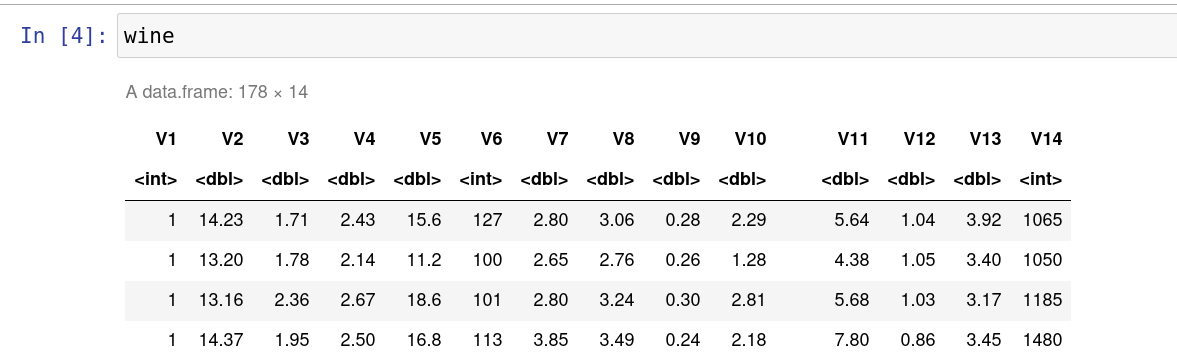
\includegraphics[width=0.8\textwidth]{dataframe_wine.png}

\begin{itemize}
\item $read.csv$ o $read.csv2$
\item $read.delim$
\end{itemize}
\end{frame}



\begin{frame}[fragile]{Media y desviación típica. Normalización.}
    \begin{columns}[c] % the "c" option specifies center vertical alignment
    \column{.5\textwidth} % column designated by a command
     \begin{lstlisting}[language=R, basicstyle=\ttfamily]
sapply(wine[2:14],mean)
V2 13.0006179775281
V3 2.33634831460674
...
V13 2.61168539325843
V14 746.893258426966 
\end{lstlisting}
    \column{.5\textwidth}
     \begin{lstlisting}[language=R, basicstyle=\ttfamily]
sapply(wine[2:14],sd)
V2 0.811826538005857
V3 1.11714609761446
...
V13 0.70999042876505
V14 314.907474276849
\end{lstlisting}



    \end{columns}
    \begin{lstlisting}[language=R, basicstyle=\ttfamily]
    standardised_wine <- as.data.frame(scale(wine[2:14]))
\end{lstlisting}
\end{frame}


\begin{frame}[fragile]{Ejemplo de selección de datos}
\small
\begin{lstlisting}
selection1 <- wine[wine$V1 == "1",]
selection3 <- wine[wine$V1 == "3",]

mean1 <- sapply(selection1[2:14],mean)
mean2 <- sapply(selection3[2:14],mean)

chemical <- c(2,3,4,5,6,7,8,9,10,11,12,13,14)
plot(chemical,mean1,col = "red")
points(chemical, mean2, col="blue", pch="*")
legend(2,1000,legend=c("Medias en Fabrica 1","Medias en Fabrica 2"), col=c("red","blue"),
                                   pch=c("o","*"))
\end{lstlisting}

\begin{wrapfigure}{r}{0.25\textwidth}
\centering
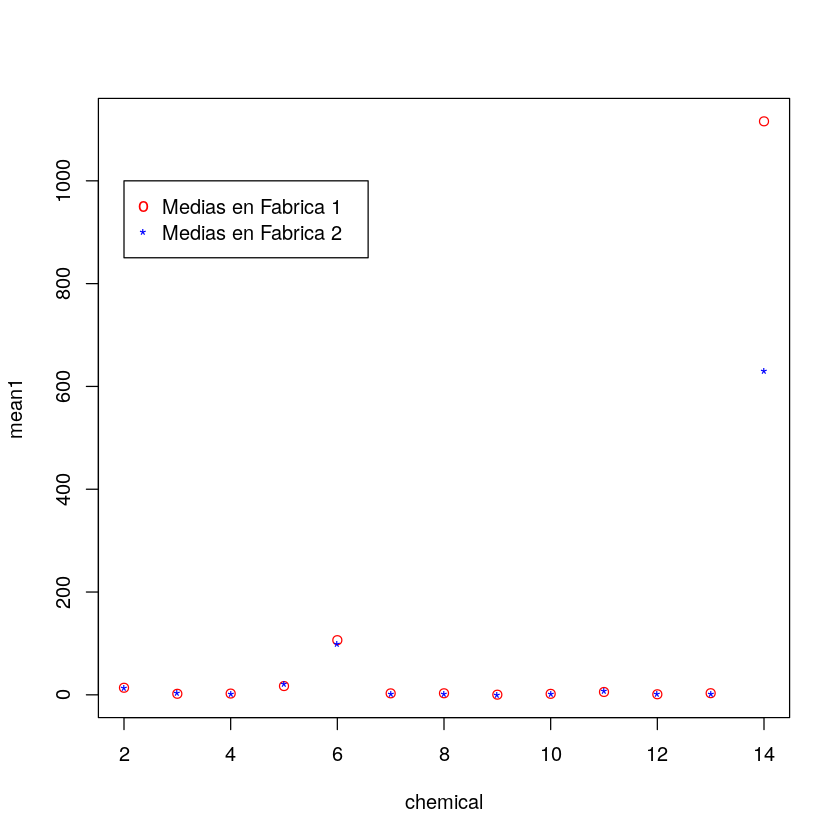
\includegraphics[width=0.8\textwidth]{means.png}
\end{wrapfigure}
\end{frame}


\begin{frame}[fragile]{Scatterplots}

Podemos realizar scatterplots de la siguiente manera



\begin{lstlisting}
plot(popul ~ manu, data = USairpollution)
\end{lstlisting}
\centering
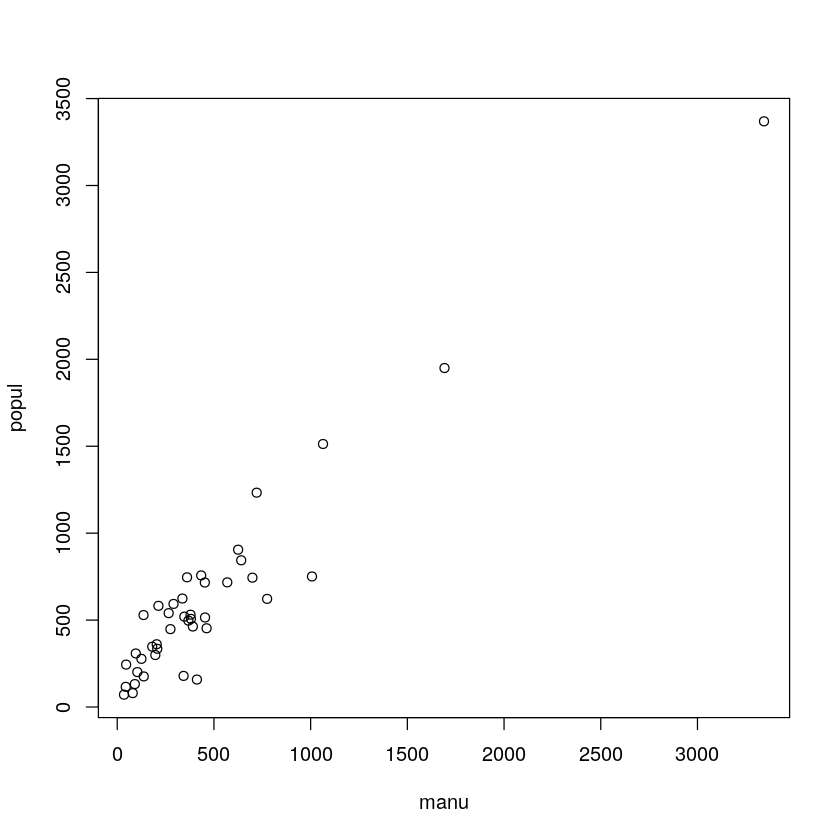
\includegraphics[width=0.4\textwidth]{scatter.png}



\end{frame}
\begin{frame}[fragile]
O, dibujar todas las parejas posibles a la vez, y añadir las rectas de regresión

\begin{lstlisting}
pairs(USairpollution,
     panel = function(x, y, ...) {
         points(x, y, ...)
         abline(lm(y ~ x), col = "grey")
     }, pch = ".", cex = 1.5)
\end{lstlisting}
\end{frame}
\begin{frame}
\centering
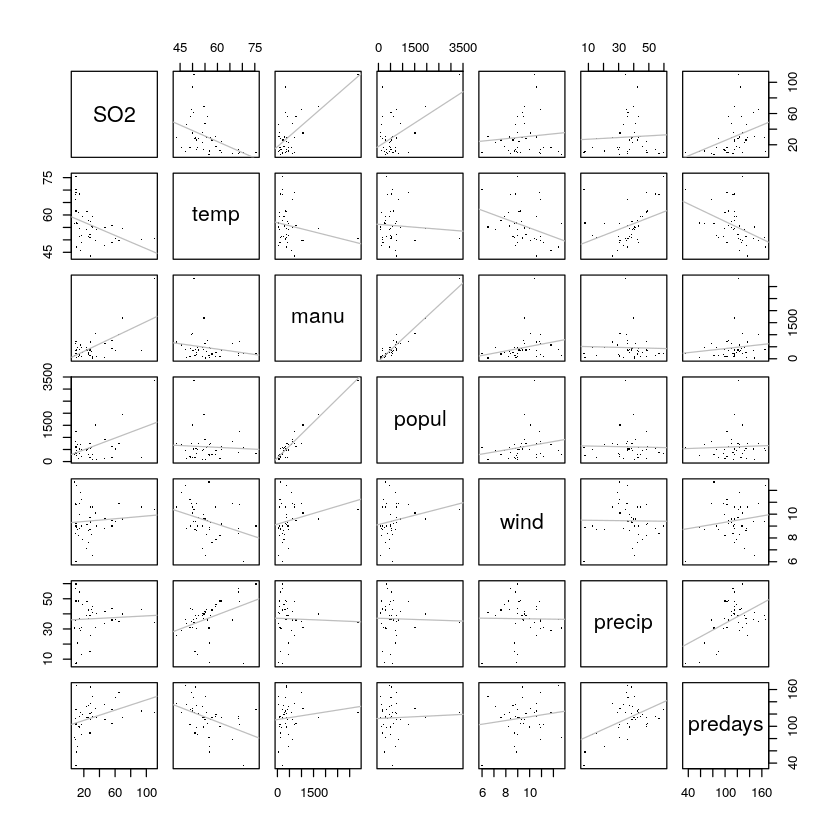
\includegraphics[width=0.7\textwidth]{reg.png}
\end{frame}


\section{Implementaciones}
\subsection{Distribución normal multivariante}
\begin{frame}[fragile]{Implementación Teórica de una DNM}

\begin{lstlisting}
DNM <- setRefClass("DNM", 
                   fields = list(p = "numeric", 
                                media = "matrix", 
                                cov = "matrix"))
\end{lstlisting}
\end{frame}


\begin{frame}[fragile]{Ejemplo de creación de una DNM}
$\pmb{X} = (X_1, X_2, X_3)^T \sim N_3 \begin{pmatrix} \begin{pmatrix} 2 \\ 3 \\ -1 \end{pmatrix}, && \begin{pmatrix} 1 & 0 & 1 \\ 0 & 5 & -2 \\ 1 & -2 & 2 \end{pmatrix} \end{pmatrix} $

\begin{lstlisting}

means <- matrix(c(2,3,-1), nrow = 3, ncol = 1)

cov <- matrix(c(1, 0, 1, 0, 5, -2, 1, -2, 2), nrow = 3, ncol = 3)

X <- DNM$new(p = 3, media = means, cov = cov); X

\end{lstlisting}
\end{frame}

\begin{frame}[fragile]{Función característica}

Implementamos la función caracteristica de la DNM $\pmb{X} = (X_1, \ldots, X_p)^T \sim N_p(\pmb{\mu}, \Sigma)$, dada por $$ \Psi_{\pmb{X}} (\pmb{t}) = \exp\left(i \pmb{t}^T \pmb{\mu} - \frac{1}{2} \pmb{t}^T \Sigma \pmb{t}\right), \; \pmb{t} \in \mathbb{R}^p $$

\scriptsize
  \begin{lstlisting}
# Pre: X es DNM, t es matriz
funcion_caracteristica <- function(X, t) {
    # Comprobacion de rango
    if (dim(t)[1] != X$p)
        stop("Filas de t no coinciden con dimension de X")
    if (dim(t)[2] != 1)
        stop("t no es vector columna")
    # psi_X(t)
    exp(as.complex(1i * t(t) %*% X$media - 0.5 * t(t) %*% X$cov %*% t))
}
  \end{lstlisting}
\end{frame}

\begin{frame}[fragile]{Función de densidad}

Implementamos la función densidad de una DNM $\pmb{X} = (X_1, \ldots, X_n)^T \sim N_p(\pmb{\mu}, \Sigma)$, con $\Sigma > 0$, que está definida para un 

$$f_{\pmb{X}}(\pmb{x}) = \dfrac{1}{(2\pi)^{p/2}|\Sigma|^{1/2}} \exp\left(-\frac{1}{2}(\pmb{x} - \pmb{\mu})^T\Sigma^{-1}(\pmb{x} - \pmb{\mu})\right), \; \pmb{x} \in \mathbb{R}^p $$

\scriptsize
  \begin{lstlisting}
# Pre: X es DNM, x matriz
funcion_densidad <- function(X, x) {
    if (dim(x)[1] != X$p)
        stop("Filas de x no coinciden con dimension de X")
    if (dim(x)[2] != 1)
        stop("x no es vector columna")
    if (det(X$cov) <= 0)
        stop("Matriz de covarianzas no es definida positiva")
    # f_X(x)
    exp(-0.5 * as.numeric(t(x - X$media) %*% solve(X$cov) %*% (x - X$media))) / ((2 * pi)^(X$p / 2) * sqrt(det(X$cov)))
}
  \end{lstlisting}
\end{frame}

\begin{frame}[fragile]{Teorema de la transformación lineal}
Necesita como argumentos una DNM $\pmb{X} \sim N_p(\pmb{\mu}, \Sigma)$, una matriz $B \in \mathcal{M}_{qxp}$ ($q \leq p$) y un vector $\pmb{b} \in \mathbb{R}^q$. Entonces devuelve la DNM definida como $\pmb{Y} = B \pmb{X} + \pmb{b}$, entonces $\pmb{Y} \sim N_q(B \pmb{\mu} + \pmb{b}, B \Sigma B^T)$.

\begin{lstlisting}
transformacion_lineal <- function(X, B, b) {
    # Comprobaciones de rango
    # Nueva DNM
    media_y = matrix(B %*% X$media + b, ncol = 1)
    cov_y = matrix(B %*% X$cov %*% t(B), nrow = dim(B)[1])
    DNM\$new(p = dim(B)[1], media = media_y, cov = cov_y)
}
\end{lstlisting}
\end{frame}
\begin{frame}[fragile]{Ejemplo}
Ejemplo con la $\pmb{X}$ anterior, $B = \begin{pmatrix} 1 & 1 & 0 \end{pmatrix}$, $b = \begin{pmatrix} 0 \end{pmatrix}$:
\begin{lstlisting}
B = matrix(c(1, 1, 0), nrow = 1, ncol = 3)
b = matrix(0, nrow = 1, ncol = 1)
Y <- transformacion_lineal(X, B, b); Y
---
Reference class object of class "DNM"
Field "p":
[1] 1
Field "media":
     [,1]
[1,]    5
Field "cov":
     [,1]
[1,]    6
\end{lstlisting}
\end{frame}


\begin{frame}[fragile]{Marginalización}
Dada una DNM $\pmb{X} = (X_1, \ldots, X_p)^T \sim N_p(\pmb{\mu}, \Sigma)$, que consiste en tomar el subvector $\pmb{X}_{\pmb{r}} = (X_{r_1}, \ldots, X_{r_q})^T$ con $\pmb{r} = (r_1, \ldots, r_q)^T, r_1, \ldots, r_q \in \{1, \ldots, q\}, q \leq p $; obteniendo $\pmb{X}_{\pmb{r}} \sim N_q(\pmb{\mu_{\pmb{r}}}, \Sigma_{\pmb{r}})$ donde:
- $\pmb{\mu_{\pmb{r}}}$ es el subvector de $\pmb{\mu}$ correspondiente a $\pmb{r}$.
- $\Sigma_{\pmb{r}}$ es la submatriz de $\Sigma$ definida por las filas y columnas correspondientes a $\pmb{r}$.
\end{frame}

\begin{frame}[fragile]

     
     \begin{lstlisting}
# Pre: X es DNM, r es matriz
marginalizar <- function(X, r) {
    # Comprobar rangos
    # mu_r
    media_r <- matrix(X$media[r, ], ncol = 1)
    # sigma_r
    cov_r <- matrix(X$cov[r, r], nrow = dim(r)[1])
    # X_r
    DNM$new(p = dim(r)[1], media = media_r, cov = cov_r)
}
\end{lstlisting}




\end{frame}

\begin{frame}[fragile]{Particionamiento independiente de una DNM}
Dada una DNM $\pmb{X} = (X_1, \ldots, X_p)^T \sim N_p(\pmb{\mu}, \Sigma)$ con $p > 1$ y $\Sigma > 0$ podemos realizar una partición de $\pmb{X} = (\pmb{X}_{(1)}^T, \pmb{X}_{(2)}^T)^T$ con $\pmb{\mu} = (\pmb{\mu}_{(1)}^T,\pmb{\mu}_{(2)}^T)^T$ y $\Sigma = \begin{pmatrix} \Sigma_{(11)} & \Sigma_{(12)} \\ \Sigma_{(21)} & \Sigma_{(22)} \end{pmatrix} $ de manera que $\pmb{X}_{(1)} = (X_1, \ldots, X_q)^T$, y $\pmb{X}_{(2)} = (X_{q+1}, \ldots, X_p)$ ($1 \leq q < p$).

\end{frame}

\begin{frame}[fragile]
\scriptsize
     \begin{lstlisting}[language=R, basicstyle=\ttfamily]
particiones_independientes <- function(X, q) {
    media_1 = matrix(X$media[1:q], ncol = 1)
    cov_11 = matrix(X$cov[1:q,1:q], nrow = q)
    X_1 <- DNM$new(p = q, media = media_1, cov = cov_11)
    # X_2 - cov_21 * cov_11^-1 * cov_12
    media_2 = matrix(X$media[(q+1):X$p], ncol=1)
    cov_22 = matrix(X$cov[(q+1):X$p, (q+1):X$p], nrow = X$p - q)
    cov_12 = matrix(X$cov[1:q, (q+1):X$p],nrow=q)
    cov_21 = matrix(X$cov[(q+1):X$p, 1:q],ncol=q)
    X_2 <- DNM$new(p = X$p - q,
                   media = media_2 - cov_21 %*% solve(cov_11) %*% media_1,
                   cov = cov_22 - cov_21 %*% solve(cov_11) %*% cov_12)
    # Devolvemos
    c(X_1, X_2)
}
\end{lstlisting}
\end{frame}

\begin{frame}{Distribución condicionada}
En las condiciones del apartado anterior, tenemos que la distribución condicionada de $\pmb{X}_{(2)}$ dado $\pmb{X}_{(1)} = \pmb{x}_{(1)}$ es una DNM con $\pmb{X}_{(2)} \sim N_{p-q}(\pmb{\mu}_{(2)}+\Sigma_{(21)} \Sigma_{(11)}^{-1}(\pmb{x}_{(1)} - \pmb{\mu}_{(1)}), \Sigma_{(22)} - \Sigma_{(21)} \Sigma_{(11)}^{-1}\Sigma_{(12)})$.

\end{frame}

\begin{frame}[fragile]
\scriptsize
\begin{lstlisting}
particion_condicionada <- function(X, q, x, dado_x2) {
    media_1 = matrix(X$media[1:q], ncol = 1)
    media_2 = matrix(X$media[(q+1):X$p], ncol = 1)
    cov_11 = matrix(X$cov[1:q,1:q], nrow = q)
    cov_22 = matrix(X$cov[(q+1):X$p, (q+1):X$p], nrow = X$p - q)
    cov_12 = matrix(X$cov[1:q, (q+1):X$p], nrow = q)
    cov_21 = matrix(X$cov[(q+1):X$p, 1:q], ncol = q)
    # DNM condicionada
    if (dado_x2) {
        p_cond = q
        media_cond = media_1 + cov_12 %*% solve(cov_22) %*% (x - media_2)
        cov_cond = cov_11 - cov_12 %*% solve(cov_22) %*% cov_21
    } else {
        p_cond = X$p - q
        media_cond = media_2 + cov_21 %*% solve(cov_11) %*% (x - media_1)
        cov_cond = cov_22 - cov_21 %*% solve(cov_11) %*% cov_12
    }
    DNM$new(p = p_cond, media = media_cond, cov = cov_cond)
}
\end{lstlisting}
\end{frame}

\subsection{Inferencia sobre DNM}

\begin{frame}[fragile]{Notacion}
Con $\pmb{X} = (X_1, \ldots, X_p)^T \sim N_p(\pmb{\mu}, \Sigma)$, $\Sigma > 0$, consideramos una muestra aleatoria simple dada por $X = (\pmb{X}_1^T, \ldots, \pmb{X}_N^T)^T$, donde N es el tamaño muestral; de manera que cada observación se representa con $\pmb{X}_\alpha, \alpha \in \{1, \ldots, N\}$.

Veremos como hacer inferencia sobre la DNM que determina $X$.
\end{frame}


\begin{frame}[fragile]{Muestra aleatoria simple}
Dada $\pmb{X} \sim N_p(\pmb{\mu}, \Sigma), \Sigma > 0$, podemos generar una muestra aleatoria simple de $\pmb{X}$ de tamaño $N$, mediante la siguiente función:

\begin{lstlisting}
muestra_aleatoria <- function(N, media, cov) {
    mvrnorm(N, media, cov)
}

muestra_aleatoria_EMV <- function(N, X) {
    mvrnorm(N, X$media, X$cov)
}
\end{lstlisting}

\end{frame}

\begin{frame}[fragile]{Muestra aleatoria simple}

Ejemplo de la m.a.s. de tamaño 14 de la DNM $\pmb{X} = (X_1, X_2, X_3)^T \sim N_3 \begin{pmatrix} \begin{pmatrix} 2 \\ 3 \\ -1 \end{pmatrix}, && \begin{pmatrix} 1 & 0 & 1 \\ 0 & 1 & -0.5 \\ 1 & -0.5 & 2 \end{pmatrix} \end{pmatrix} $:

\begin{lstlisting}
X_DNM <- DNM$new(p = 3,
          media = matrix(c(2,3,-1), ncol = 1),
          cov = matrix(c(1,0,1,0,1,-0.5,1,-0.5, 2), ncol = 3, nrow = 3))
X <- muestra_aleatoria_EMV(20, X_DNM); X[1:10,]
\end{lstlisting}

\end{frame}

\begin{frame}[fragile]{Muestra aleatoria simple}

\begin{center}
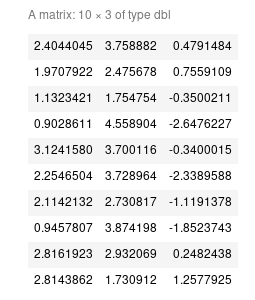
\includegraphics[scale=0.7]{mas.png}
\end{center}

\end{frame}

\begin{frame}[fragile]{Media muestral}
Implementamos la media muestral $\pmb{\bar{X}} = \frac{1}{N} \sum^N_{\alpha = 1} \pmb{X}_\alpha = \begin{pmatrix} \bar{X}_1 \\ \vdots \\ \bar{X}_p \end{pmatrix}$

Además este es el estimador máximo verosímil ($\pmb{\hat{\mu}} = \pmb{\bar{X}}$).

\begin{lstlisting}
media_muestral <- function(X) {
    matrix(colMeans(X), ncol = 1)
}
\end{lstlisting}

\end{frame}

\begin{frame}[fragile]{Media muestral}

Ejemplo con $X$ anterior:

\begin{lstlisting}
media_muestral(X)
\end{lstlisting}

\begin{center}
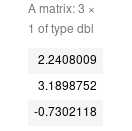
\includegraphics[scale=0.7]{media_muestral.png}
\end{center}


\end{frame}

\begin{frame}[fragile]{Matrices muestrales}

Implementamos las siguientes matrices:

\begin{itemize}

\item Matriz de dispersiones muestral: $A = \sum^N_{\alpha = 1} (\pmb{X}_\alpha - \pmb{\bar{X}})(\pmb{X}_\alpha - \pmb{\bar{X}})^T$
\item Matriz de covarianzas muestral: $S_N = \frac{1}{N} A$
\item Matriz de cuasi-covarianzas muestral: $S_{N+1} = \frac{1}{N-1} A $ (también llamada matriz de covarianzas muestral)
\item Matriz de correlaciones muestral: $R = D^{1/2}S_N D^{-1/2}$, donde $D$ es la diagonal de $S_N$

\end{itemize}

Sabemos que $\hat{\Sigma} = S_N$, $T = S_{N+1}$ es estimador eficiente de $\Sigma$, y $\hat{p} = R$ (coeficientes de correlacion lineal de Pearson).

\end{frame}


\begin{frame}[fragile]{Matrices muestrales}

\begin{lstlisting}
disp_muestral <- function(X) {
    cov(X) * (nrow(X) - 1)
}

cov_muestral <- function(X) {
    disp_muestral(X) / nrow(X)
}

cuasicov_muestral <- function(X) {
    disp_muestral(X) / (nrow(X)-1)
}

cor_muestral <- function(X) {
    cor(X)
}
\end{lstlisting}

\end{frame}

\begin{frame}[fragile]{Matrices muestrales}

Ejemplo con la $X$ anterior:

\small
\begin{lstlisting}
print(disp_muestral(X))
print(cov_muestral(X))
print(cuasicov_muestral(X))
print(cor_muestral(X))
\end{lstlisting}

\scriptsize
\begin{lstlisting}
          [,1]      [,2]      [,3]
[1,] 21.479470 -1.012076 22.441216
[2,] -1.012076 18.552064 -9.202547
[3,] 22.441216 -9.202547 39.923667
           [,1]       [,2]       [,3]
[1,]  1.0739735 -0.0506038  1.1220608
[2,] -0.0506038  0.9276032 -0.4601274
[3,]  1.1220608 -0.4601274  1.9961834
            [,1]        [,2]       [,3]
[1,]  1.13049840 -0.05326715  1.1811166
[2,] -0.05326715  0.97642444 -0.4843446
[3,]  1.18111663 -0.48434460  2.1012456
            [,1]        [,2]       [,3]
[1,]  1.00000000 -0.05069968  0.7663363
[2,] -0.05069968  1.00000000 -0.3381401
[3,]  0.76633630 -0.33814014  1.0000000
\end{lstlisting}
\end{frame}

\begin{frame}[fragile]{Contraste sobre $\pmb{\mu}$}

Sobre $\pmb{X} \sim N_p(\pmb{\mu}, \Sigma)$, $\Sigma>0$ y $\{\pmb{X}_{\alpha} : \alpha = 1, \ldots, N\}$, con $N > p$ una m.a.s de $\pmb{X}$ nos planteamos el problema de contrastre $$\begin{cases} H_0 : \pmb{\mu} = \pmb{\mu}_0 \\ H_1: \pmb{\mu} \neq \pmb{\mu}_0 \end{cases}, \pmb{\mu}_0 \in \mathbb{R}^p \text{ dado.} $$
\end{frame}

\begin{frame}[fragile]{$\Sigma$ conocida}

Usamos estadístico de Wishart $W = N (\pmb{\bar{X}} - \pmb{\mu}_0)^T \Sigma^{-1} (\pmb{\bar{X}} - \pmb{\mu}_0) $ sigue una $\chi^2_p(\delta)$ con $\delta = N (\pmb{\mu} - \pmb{\mu}_0)^T \Sigma^{-1} (\pmb{\mu} - \pmb{\mu}_0)$, y la función test para el problema es:

$$ \Phi(X) = \begin{cases} 1 \text{ si } W > \chi^2_{p;\alpha} \\ 0 \text{ si } W \leq \chi^2_{p;\alpha} \end{cases}, $$

donde $\chi^2_{p;\alpha}$ representa el valor de una distribución $\chi^2_p$ que deja a su derecha una probabilidad $\alpha$.

En nuestro caso si no proporcionamos la probabilidad $\alpha$ nos devolverá el p-value, que es la probabilidad que deja $W$ a su derecha.

\end{frame}

\begin{frame}[fragile]{$\Sigma$ conocida}
\begin{lstlisting}
media_test_sigma <- function(X, media_0, cov, alpha = NA) {
    N <- nrow(X)
    p <- ncol(X)
    media <- media_muestral(X)
    W <- N * (t(media - media_0) %*% solve(cov) %*% (media - media_0))
    p_value <- 1 - pchisq(W, p)
    if (!is.na(alpha))
        cat("\nResultado del test: ", as.logical(p_value < alpha))
    else
        cat("\np-value: ", p_value)
}
\end{lstlisting}
\end{frame}

\begin{frame}[fragile]{$\Sigma$ conocida}

Probamos el test con el $X$ anterior:

\scriptsize
\begin{lstlisting}
print(X_DNM$media)
print(media_muestral(X))
media_test_sigma(X, X_DNM$media, X_DNM$cov)
media_test_sigma(X, media_muestral(X), X_DNM$cov)
media_test_sigma(X, c(2.5, 3.5, -1.2), X_DNM$cov)
media_test_sigma(X, X_DNM$media, X_DNM$cov, alpha = 0.05)
\end{lstlisting}

\scriptsize
\begin{lstlisting}
     [,1]
[1,]    2
[2,]    3
[3,]   -1
           [,1]
[1,]  2.2408009
[2,]  3.1898752
[3,] -0.7302118

p-value:  0.5143849
p-value:  1
p-value:  0.007210622
Resultado del test:  FALSE
\end{lstlisting}


\end{frame}


\begin{frame}[fragile]{$\Sigma$ desconocida}
Usamos el estadístico de $T^2$ de Hotelling, con $T^2 = N (\pmb{\bar{X}} - \pmb{\mu}_0)^T S_{N-1}^{-1} (\pmb{\bar{X}} - \pmb{\mu}_0)$, donde $\dfrac{T^2}{N-1} \dfrac{N-p}{p} \sim F_{p;N-p}(\delta)$ con $\delta = N (\pmb{\mu} - \pmb{\mu}_0)^T \Sigma^{-1} (\pmb{\mu} - \pmb{\mu}_0)$, y entonces la función test para el problema es:

$$ \Phi(X) = \begin{cases} 1 \text{ si } (N-p)T^2 > (N-1)pF_{p;N-p;\alpha} \\ 0 \text{ si } (N-p)T^2 \leq (N-1)pF_{p;N-p;\alpha} \end{cases}, $$

donde $F_{p;N-p;\alpha}$ representa el valor de una distribución $F_{p;N-p}$ que deja a su derecha una probabilidad $\alpha$.
\end{frame}


\begin{frame}[fragile]{$\Sigma$ desconocida}

\begin{lstlisting}
media_test <- function(X, media_0, alpha = NA) {
    N <- nrow(X)
    p <- ncol(X)
    media <- media_muestral(X)
    S <- cuasicov_muestral(X)
    T <- N * (t(media - media_0) %*% solve(S) %*% (media - media_0))
    T_val <- T * (N - p) / (p * (N - 1))
    p_value <- 1 - pf(T_val, p, N - p)
    if (!is.na(alpha))
        cat("\nResultado del test: ", as.logical(p_value < alpha))
    else
        cat("\np-value: ", p_value)
}

\end{lstlisting}

\end{frame}

\begin{frame}[fragile]{$\Sigma$ desconocida}

Probamos con $X$:

\scriptsize
\begin{lstlisting}
print(X_DNM$media)
print(media_muestral(X))
media_test(X, X_DNM$media)
media_test(X, media_muestral(X))
media_test(X, c(2.1, 3.1, -1.2))
media_test(X, c(3, 0, 0), alpha = 0.05)
\end{lstlisting}

\scriptsize
\begin{lstlisting}
     [,1]
[1,]    2
[2,]    3
[3,]   -1
           [,1]
[1,]  2.2408009
[2,]  3.1898752
[3,] -0.7302118

p-value:  0.5912787
p-value:  1
p-value:  0.2963594
Resultado del test:  TRUE
\end{lstlisting}

\end{frame}


\begin{frame}[fragile]{Superficies de confianza}

Ahora nos planteamos como representar las superficies de confianza de $\mu$, es decir, dada $X_i$, $X_j$ de $\pmb{X}$ la región de $\mathbb{R}^2$ donde se pueda encontrar $\mu$ con cierta probabilidad $1 - \alpha$.

\end{frame}

\begin{frame}[fragile]{$\Sigma$ conocida}

Para formar las regiones de confianza para el vector de medias $\pmb{\mu}$ consideramos que:

$$P[W \leq  \chi^2_{p;\alpha}]= 1 - \alpha,$$
donde $W$ era el estadístico de Wishart definido en el test de contraste.

Tenemos entonces que la región de confianza al $100(1 - \alpha)\%$ del vector de medias $\pmb{\mu}$ está definida por todos los $\pmb{\mu}_0 \in \mathbb{R}^p$ tales que cumplen:

$$N (\pmb{\bar{X}} - \pmb{\mu}_0)^T \Sigma^{-1}(\pmb{\bar{X}} - \pmb{\mu}_0) \leq \chi^2_{p;\alpha}$$

Se representa como elipse, con $\Sigma$ y $\sqrt{\dfrac{1}{N} \chi^2_{p;\alpha}}$.

\end{frame}

\begin{frame}[fragile]{$\Sigma$ conocida}

\begin{lstlisting}
elipse_medias_sigma <- function(X, id, cov, alpha, col = "black", pch = 1, draw = FALSE) {
    p <- ncol(X)
    N <- nrow(X)
    media <- media_muestral(X)
    radio <- sqrt(qchisq(alpha,p) / N)
    elipse <- ellipse(center = media[id], shape = cov[id,id], radius = radio, draw = FALSE, pch = pch, col = col)
    if (!draw)
        plot(elipse, pch = pch, col = col)
    else
        points(elipse, pch = pch, col = col)
    points(matrix(media[id], ncol = 2), pch = 2, col = "red")
}
\end{lstlisting}
\end{frame}


\begin{frame}[fragile]{$\Sigma$ conocida}

Ejemplo con $X$ con $\alpha = 0.99, 0.95, 0.90$:

\begin{lstlisting}

plot(X[, c(1,3)], xlab = "1", ylab = "3")
elipse_medias_sigma (X, c(1,3), X_DNM$cov, 0.99, col = "orange", draw = TRUE)
points(matrix(X_DNM$media[c(1,3)], ncol=2), pch = 1, col = "blue")
elipse_medias_sigma (X, c(1,3), X_DNM$cov, 0.90, col = "green", pch = 1, draw = TRUE)
elipse_medias_sigma (X, c(1,3), X_DNM$cov, 0.95, col = "yellow", pch = 1, draw = TRUE)

\end{lstlisting}

\end{frame}

\begin{frame}[fragile]{$\Sigma$ desconocida}

\begin{center}
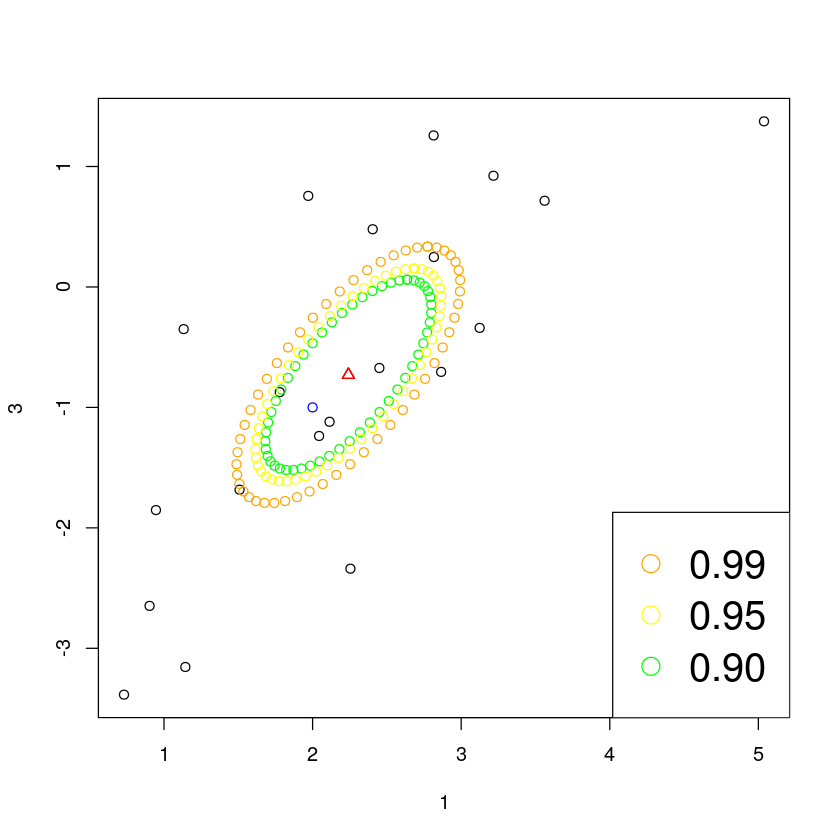
\includegraphics[scale=0.4]{superficie1.png}
\end{center}
\end{frame}


\begin{frame}[fragile]{$\Sigma$ desconocida}

Para formar las regiones de confianza para el vector de medias $\pmb{\mu}$ consideramos que:

$$P\left[T^2 \leq \dfrac{p(N-1)}{N-p} F_{p;N-p;\alpha}\right]= 1 - \alpha,$$
donde $T^2$ era el estadístico de Hotelling definido en el test de contraste.

Tenemos entonces que la región de confianza al $100(1 - \alpha)\%$ del vector de medias $\pmb{\mu}$ está definida por todos los $\pmb{\mu}_0 \in \mathbb{R}^p$ tales que cumplen:

$$N (\pmb{\bar{X}} - \pmb{\mu}_0)^T S_{N-1}^{-1}(\pmb{\bar{X}} - \pmb{\mu}_0) \leq \dfrac{p(N-1)}{N-p} F_{p;N-p;\alpha} $$

Se representa como elipse, usando $S_{N-1}$ y $\sqrt{\dfrac{p(N-1)}{N(N-p)} F_{p;N-p;\alpha}}$.

\end{frame}



\begin{frame}[fragile]{$\Sigma$ desconocida}

\begin{lstlisting}
elipse_medias <- function(X, id, alpha, col, pch, draw) {
    p <- ncol(X)
    N <- nrow(X)
    media <- media_muestral(X)
    S <- cuasicov_muestral(X)
    radio <- sqrt(p*(N-1)*qf(alpha,p,N-p)/(N*(N-p)))
    elipse <- ellipse(center = media[id], 
      shape = S[id,id], radius = radio, draw = FALSE, pch = pch, col = col)
    plot(elipse)
    points(matrix(media[id], ncol = 2), pch = 2, col = "red")
}
\end{lstlisting}

\end{frame}


\begin{frame}[fragile]{$\Sigma$ desconocida}

\begin{lstlisting}
plot(X[, c(1,3)], xlab = "1", ylab = "3")
elipse_medias(X, c(1,3), 0.99, col = "orange", draw = TRUE)
points(matrix(X_DNM$media[c(1,3)], ncol=2), pch = 3, col = "blue")
elipse_medias(X, c(1,3), 0.90, col = "green", pch = 10, draw = TRUE)
elipse_medias(X, c(1,3), 0.95, col = "yellow", pch = 5, draw = TRUE)
\end{lstlisting}

\end{frame}


\begin{frame}[fragile]{$\Sigma$ desconocida}

\begin{center}
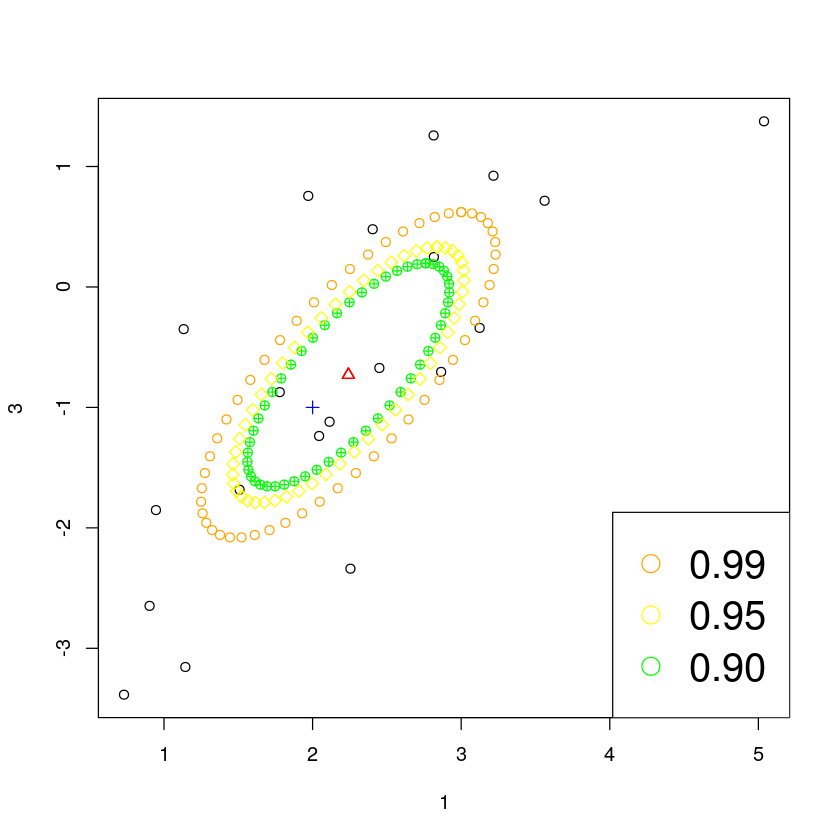
\includegraphics[scale=0.4]{superficie2.png}
\end{center}
\end{frame}


\section{Bibliografía}
\begin{frame}{Bibliografía}
\textit{Using R for Data Analysis and Graphics. Introduction, Code and Commentary} J.H. Maindonald (2004)
\newline
\newline
\textit{Applied Predictive Modeling} Max Kuhn \& Kjell Johnson (2013)
\newline
\newline
\textit{An Introduction to Statistical Learning with Applications in R} Gareth James, Daniela Witten, Trevor Hastie \& Robert Tibshirani (6th printing 2015)
\newline
\newline
\textit{The Elements of Statistical Learnig. Data Mining, Inference, and Prediction.} Trevor Hastie, Robert Tibshirani \& Jerome Friedman (2nd edition 2001)
\newline
\newline
\textit{An Introduction to Applied Multivariate Analysis with R.} Brian Everitt \& Torsten Hothorn (2011)
\end{frame}

\begin{frame}{Biliografía}
\textit{R-Forge} (Consultado 21/01/2020)
\\\texttt{http://r-forge.r-project.org/}
\newline
\newline
\textit{Cran R Contributed Packages} (Consultado 21/01/2020)
\\\texttt{https://cran.r-project.org/web/packages/}
\newline
\newline
\textit{Cran R Contributed Packages Captura Diciembre 2019}
\\\texttt{https://web.archive.org/web/20191210081209/http://
cran.r-project.org/web/packages}
\newline
\newline
\textit{Cran R Task Views} (Consultado 21/01/2020)
\\\texttt{https://cran.r-project.org/web/views/}
\newline
\newline
\textit{Tutorialspoint} (Consultado 21/01/2020)
\\\texttt{https://www.tutorialspoint.com/r/index.htm}
\end{frame}
\end{document}
